\subsubsection{Definition of inputs and outputs of the neural networks}\label{inputs-outputs}

Before continuing to explain the steps carried out, the structure of the dataset needed to train the neural networks must be defined. One of the main requirements in neural network design is the correct specification of the input and output vector of the neural network. The number of variables and the type of variables that will be used in the network is one of the main keys for the model to work satisfactorily. In this section both the structure of the input vector and the structure of the output vector will be explained with graphic examples.
\newline

The models worked with will have values in the input vector representing the date and time represented with the following attributes: \small{\verb|hour|} \normalsize ($h$), \small{\verb|day_of_week|} \normalsize ($d$) and \small{\verb|month|} \normalsize ($m$). To do this, it is necessary that the trips are grouped by intervals, thus creating new columns(\textit{quantity\_$j$}), where $j$ is an integer that represents the station identifier within the network. These columns will be referenced with a $q$. In total there are $633$ stations in the city of Chicago. So for each interval, the neural network will have $636$ input values. You can see graphic examples in figure \ref{fig:models-design-1} and \ref{fig:models-design-2}. The size of the final dataset will be \small\verb|n_intervals| $\times ($ \small\verb|n_stations| $+ 3)$\normalsize.
\newline

The most basic thing would be to create a model that takes a single interval as input and predicts a single interval represented by the output vector. For this model, the network input would be $636$, formed by $[h, d, m, q_j], j$ $ \forall$ $[1, 633]$, where $h$, $d$ and $m$ are the three variables that provide information about the interval and \textit{$q_j, j\in [1, 633]$}] are values that represent the number of trips initiated for station $j$  in that interval. The output would be a vector of $633$ elements that would represent the prediction of the interval immediately after the input interval and would have the same order as the input vector \textit{quantity\_$j, j\in [1, 633]$}.
\newline

If you want to use more intervals in the model, the input vector will have a number of elements multiple of $636$. For example, if you want to use 5 intervals as input vector, then the network will have a first layer with $636 \times 5 = 3180$ units or neurons. Similarly, if you want the output of the network to be a vector containing the prediction for all the stations in the network, the size of the resulting vector will be a multiple of $633$.
\newline


In \acrfull{ar} models, despite being models capable of predicting multiple intervals if necessary, the output of these models will always be an interval. This is because it is necessary to calculate all the intervals independently because the \acrshort{ar} model uses its own prediction as an input vector. More information on this can be seen in section \ref{window_ar} and \ref{model_ar}.
\newline

Below, several examples of different network configurations using different combinations for the number of input and output intervals can be seen graphically:

\begin{figure}[H]
    \centering
    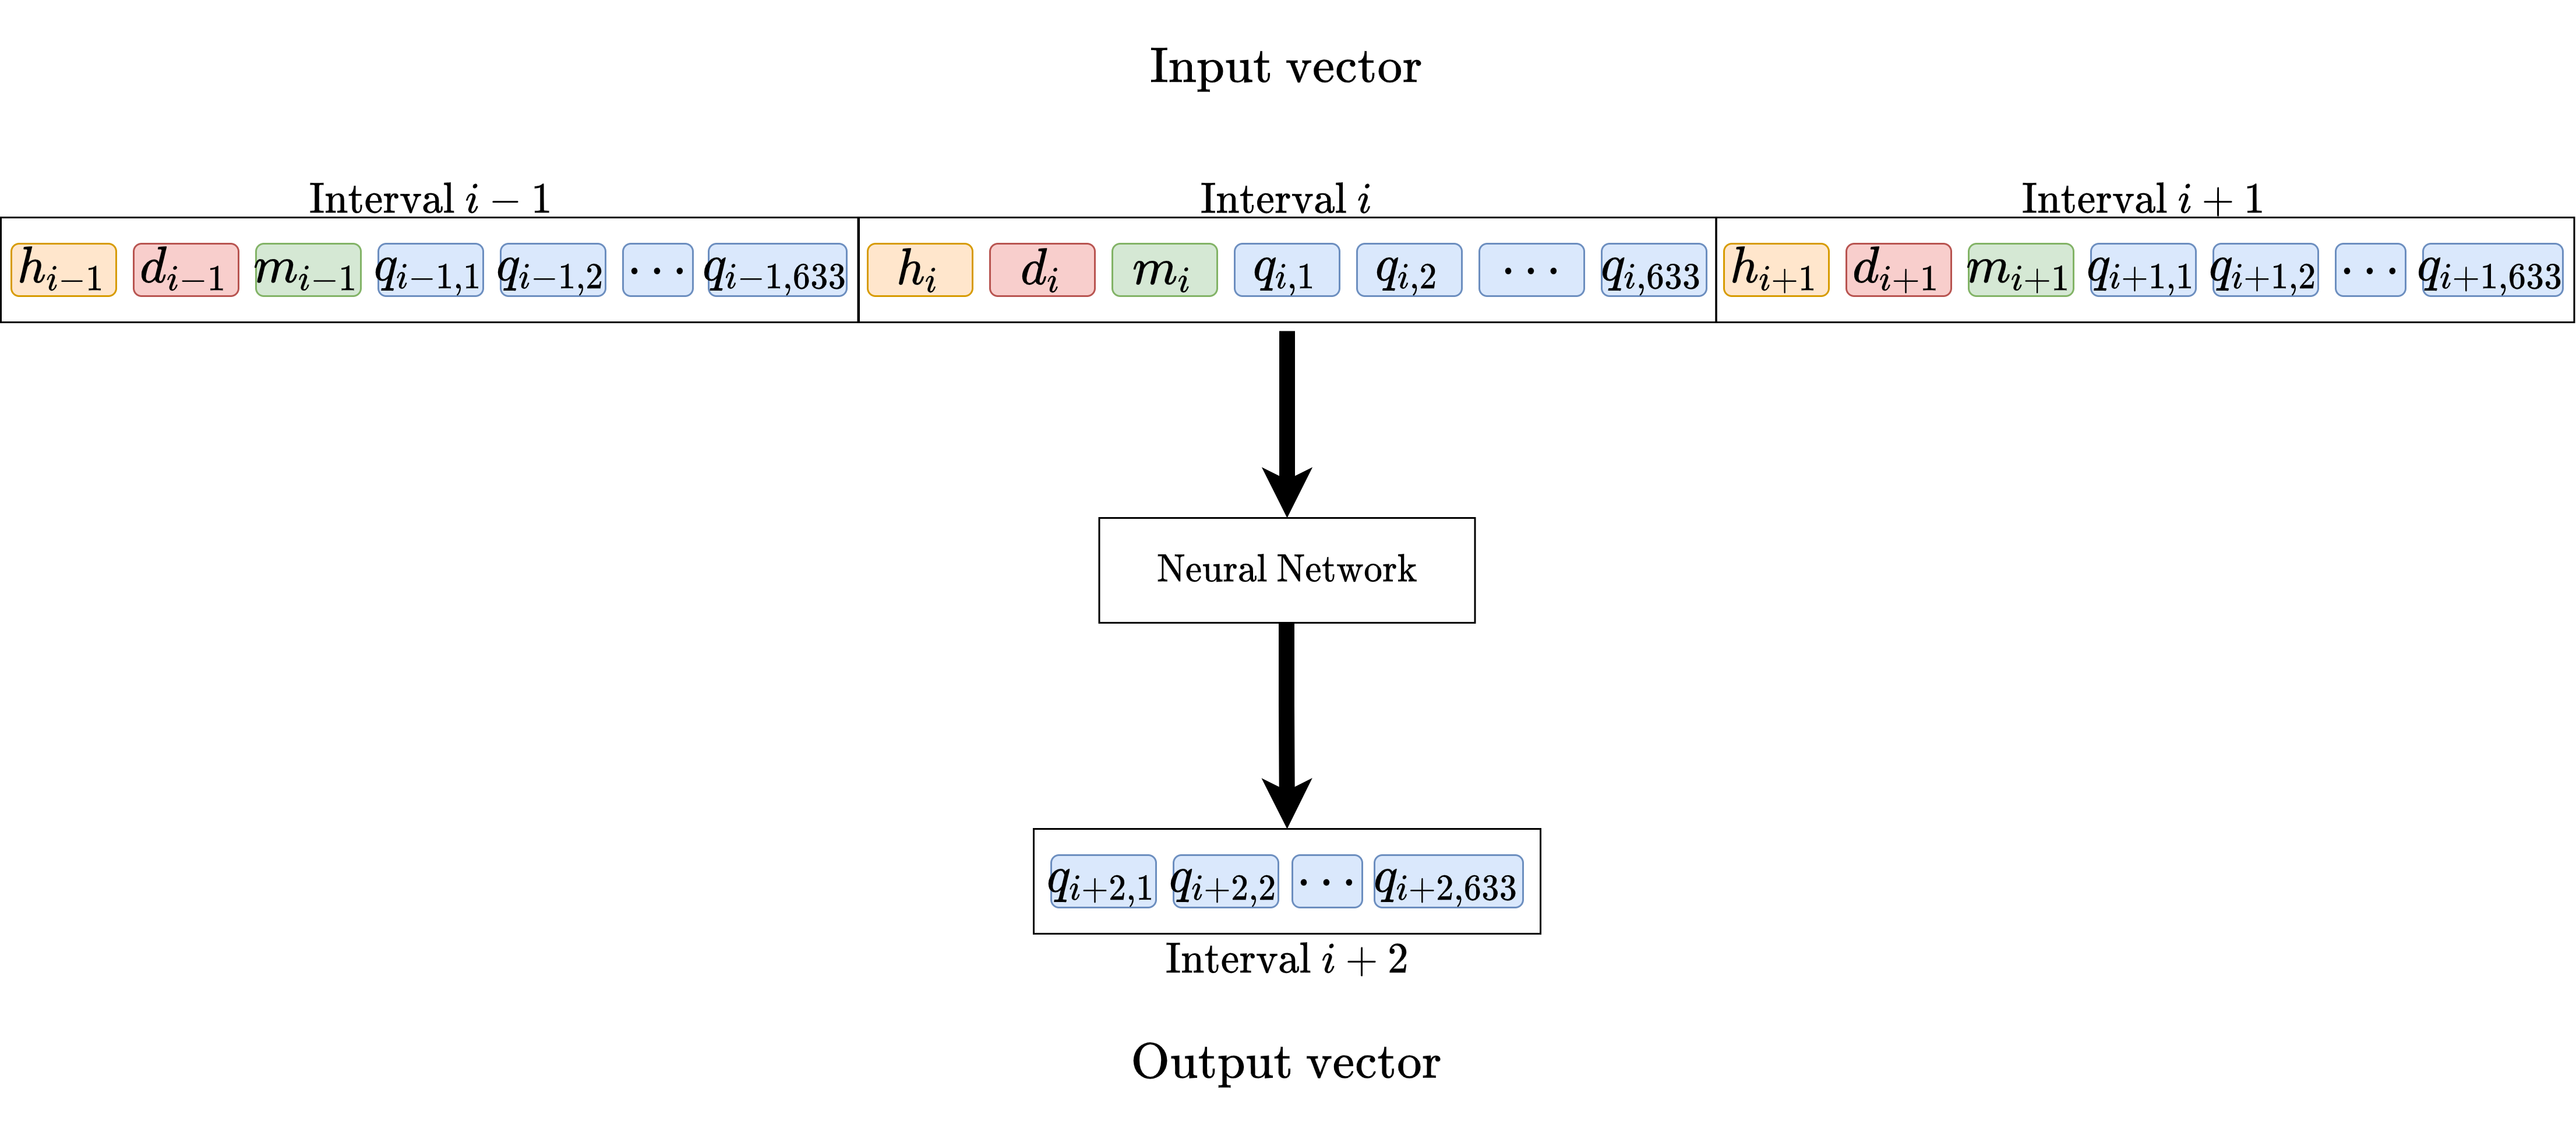
\includegraphics[width=14cm]{images/solution/preprocessing/models-design-1.png}
    \caption{Example of a neural network using 3 input intervals and predicting 1 interval.}
    \label{fig:models-design-1}
\end{figure}

\begin{figure}[H]
    \centering
    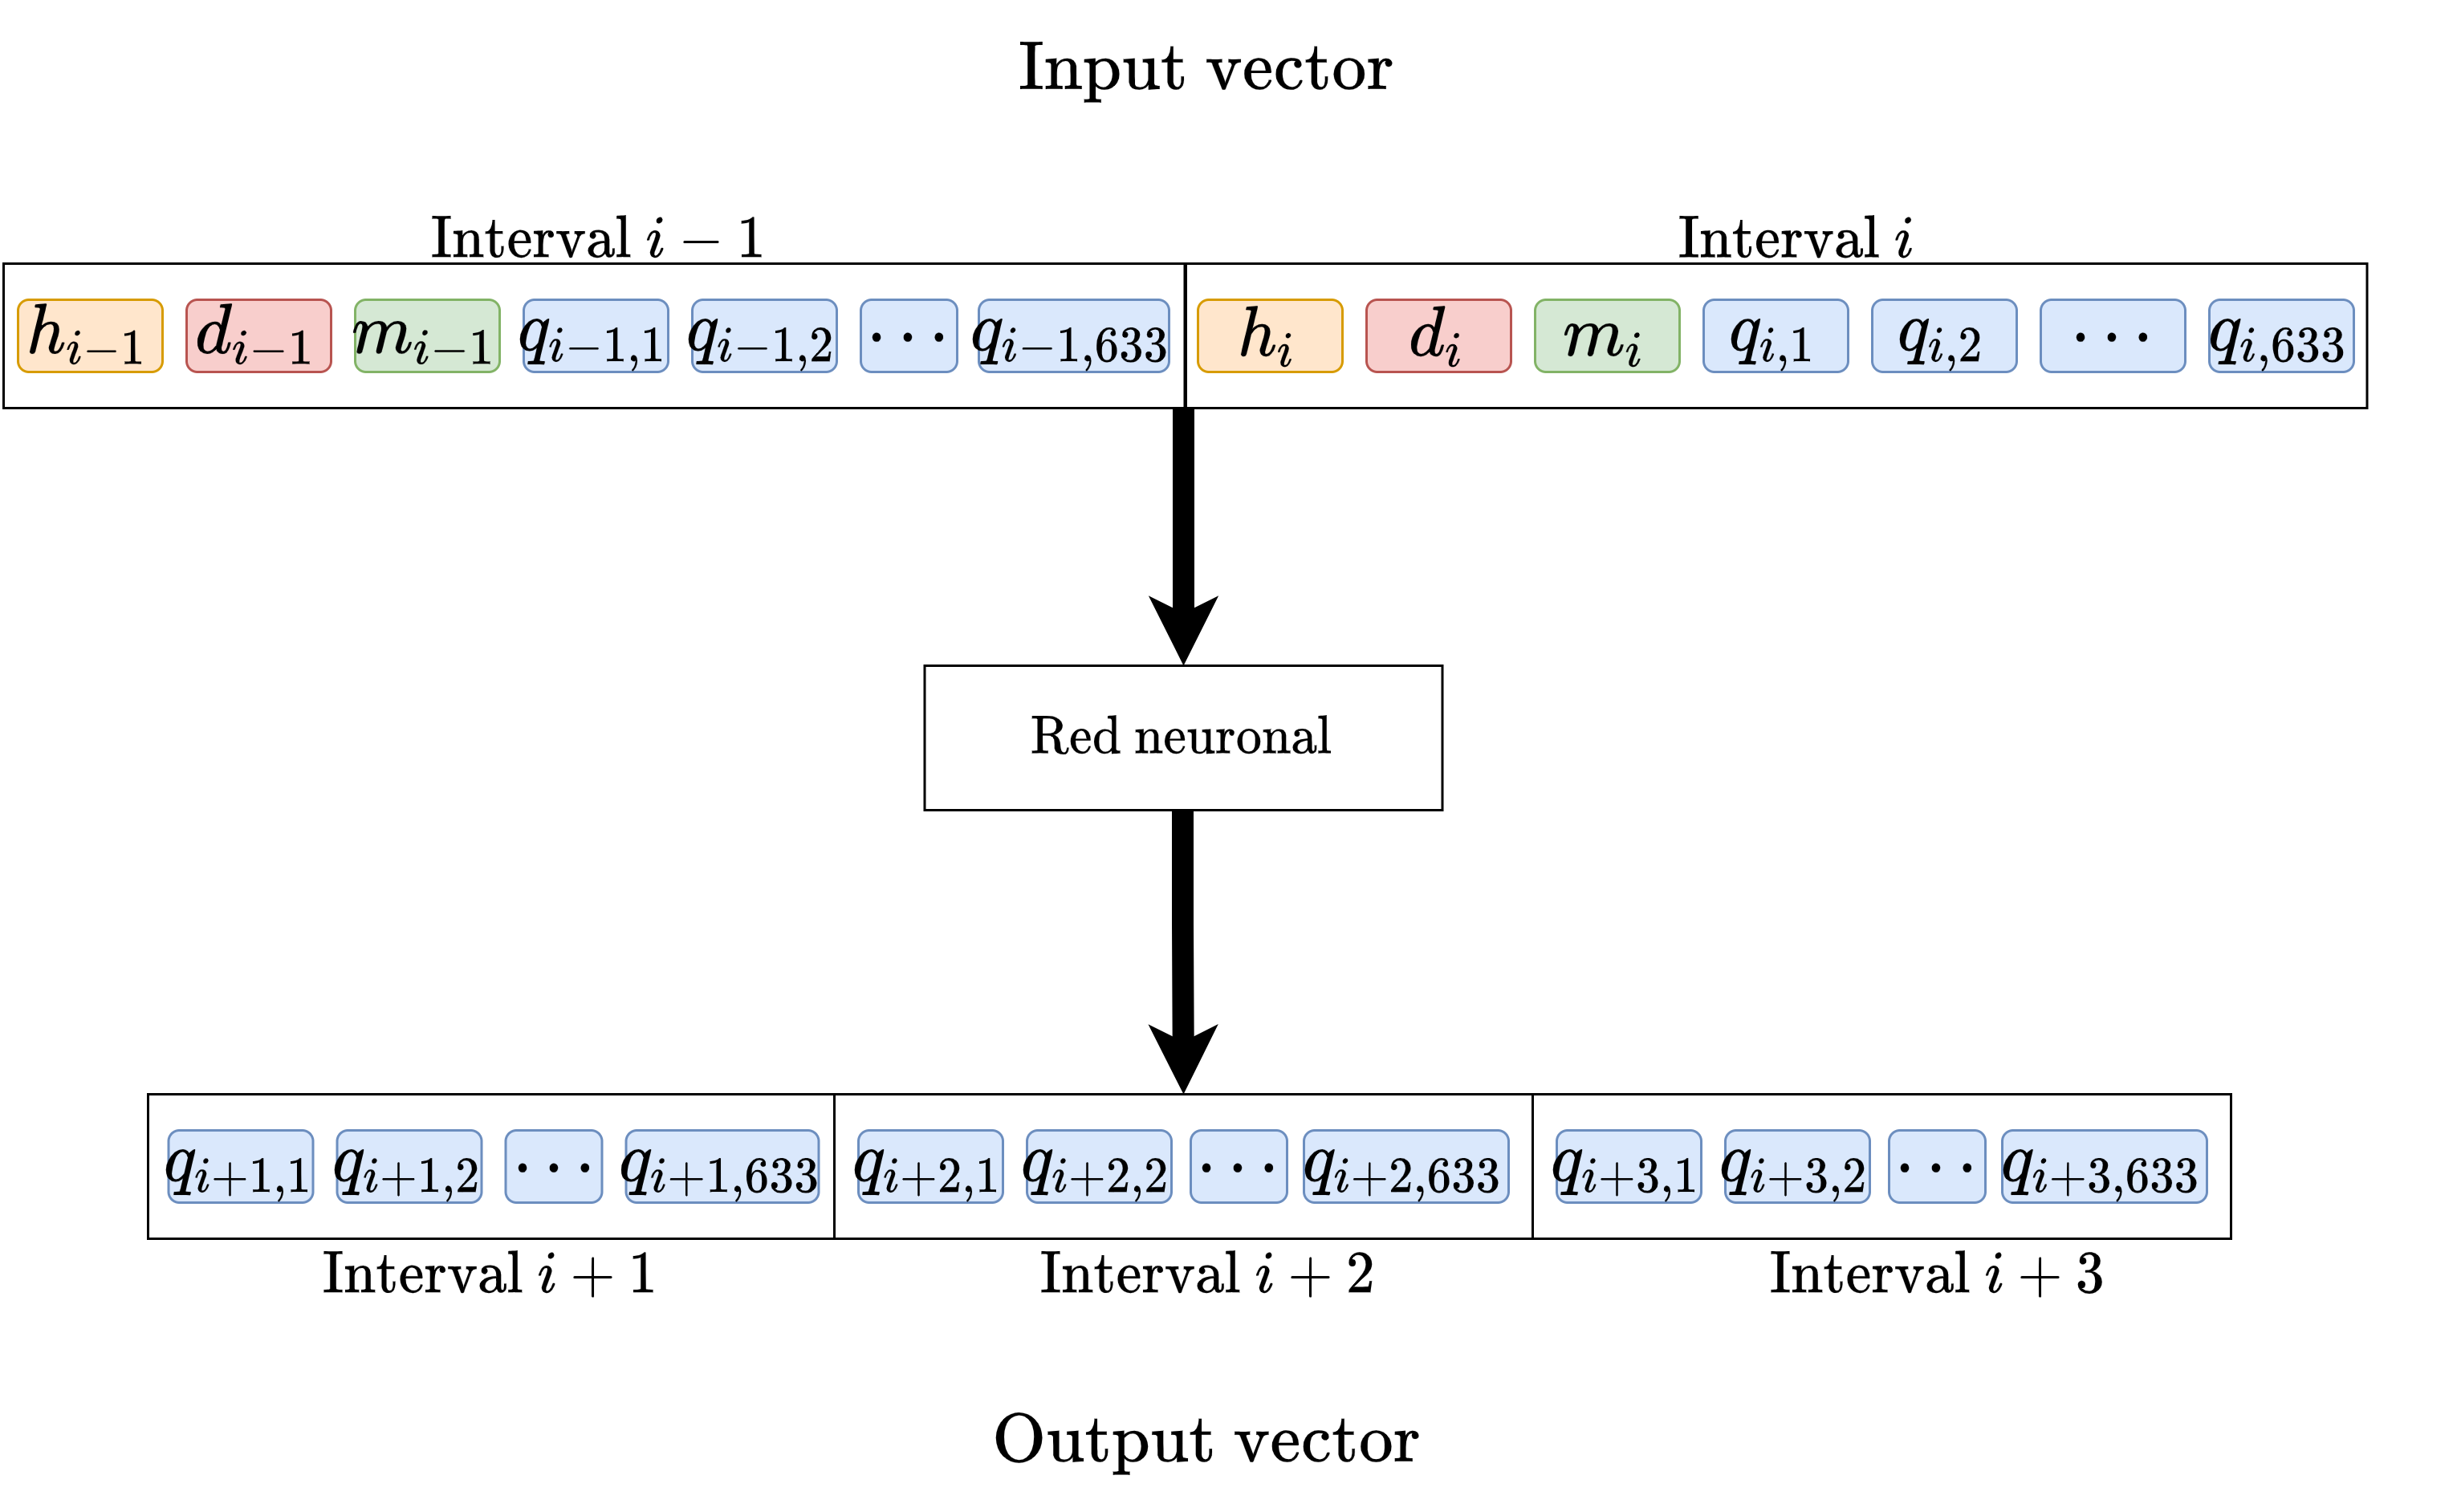
\includegraphics[width=14cm]{images/solution/preprocessing/models-design-2.png}
    \caption{Example of a neural network using 2 input intervals and predicting 3 intervals.}
        \label{fig:models-design-2}
\end{figure}


This way of structuring data and models is very flexible. It allows the code to be easily adapted to other datasets and is not unique to the city of Chicago. In addition, it also allows you to work with a smaller group of stations if you wish. As each column is a station, simply by filtering through the columns that are of interest, the models could be trained with these columns. It would also be possible to work by communities, grouping the stations according to a series of rules and thus be able to study the patterns of a neighbourhood and not of each station in a particular way as is done in this work.
\newline